\section{仿真结果与分析}
\subsection{主观评价}

去雾的图片来自于RESIDE\cite{li2019benchmarking}的HSTS数据集,从图\ref{fig-dehazy}的效果来看,不同的去雾算法都实现了去雾的功能。SID方法都基于强大的假设和先验。这些方法只有在假设为真时才会表现良好。由于这些假设或先验的失败,SID 方法缺乏准确性。通常,通过使用平滑来提高传输的精度,然后降低去雾的计算速度。此外,可以使用先验或通过估计无雾图像的最小颜色通道来估计透射率。先验只有在假设为真时才会表现良好,而最小颜色通道的估计误差会随着雾度密度的增加而增加。这种不准确会导致可见度降低和颜色失真。从图上看前几种算法就出现了可见度降低和颜色失真,即便由于超参设置问题它们在后面的PSNR与SSIM指标中比NLB的方法更高(理论上客观指标也是最高的),主观感受中NLB的方法也是最佳的。

\begin{figure}[htbp]
    \centering
    \subfloat[有雾图]{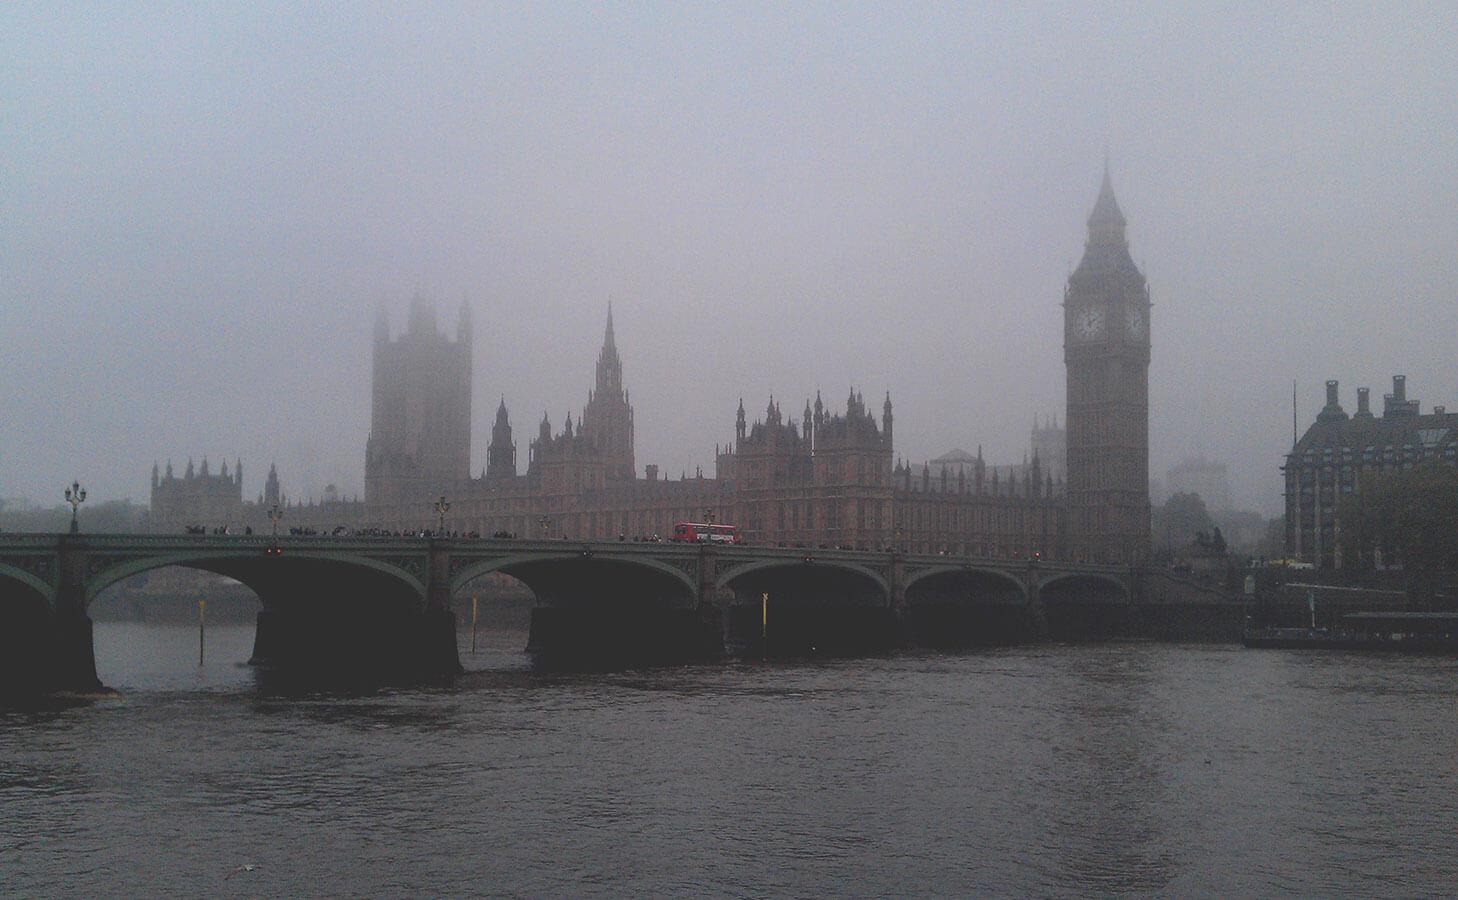
\includegraphics[width=0.3\textwidth]{../data/HSTS_real-world/HazyDr_Google_396.jpeg}}\quad
    \subfloat[DCP
        ]{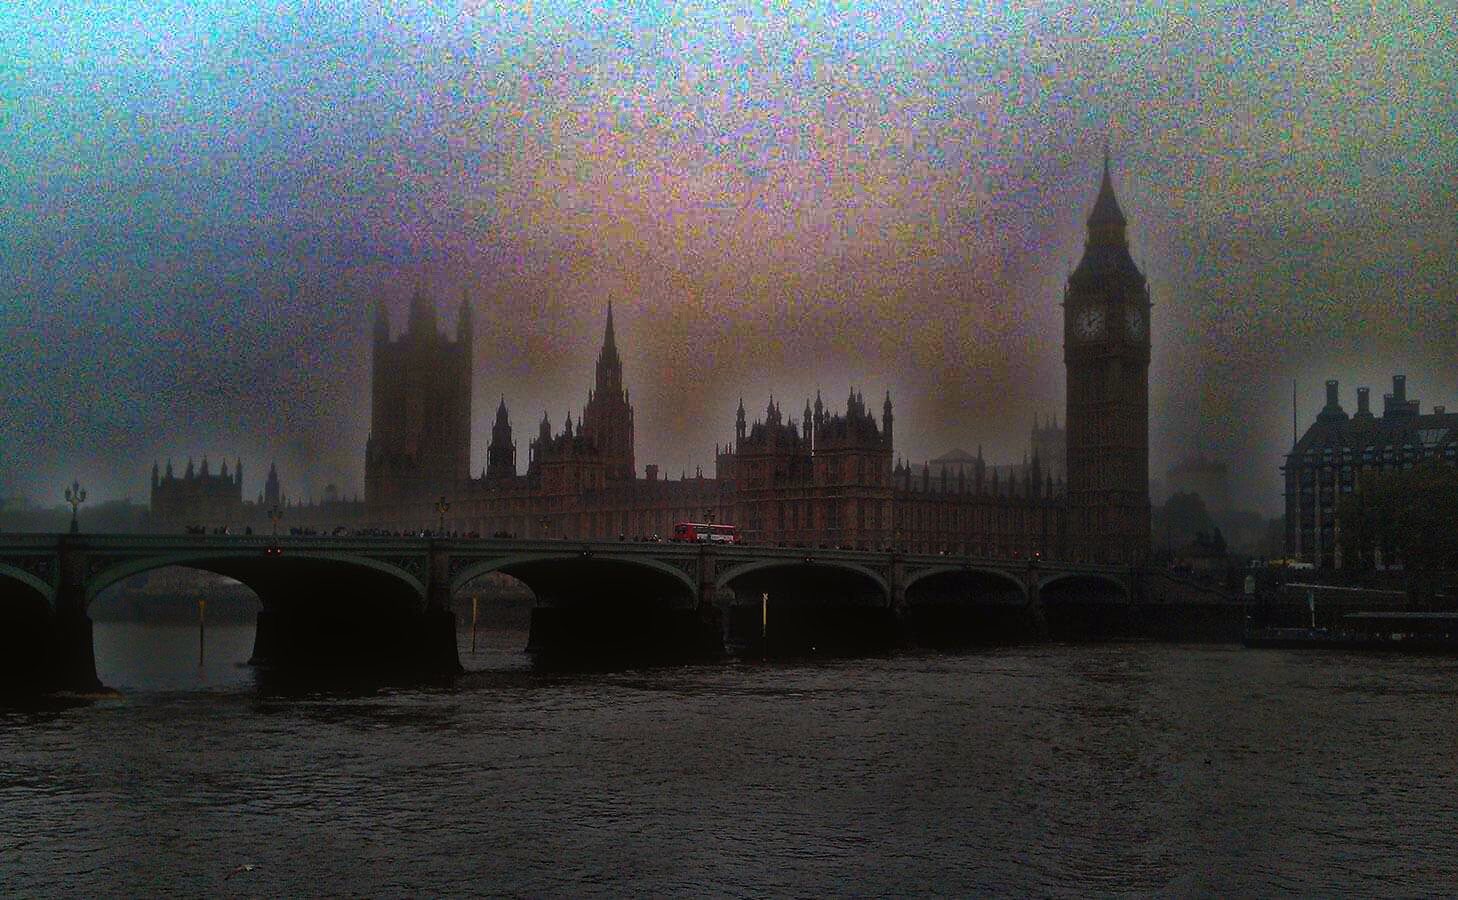
\includegraphics[width=0.3\textwidth]{../output/HSTS_real-world/H_HazyDr_Google_396.jpeg}}
    \quad\subfloat[BCL]{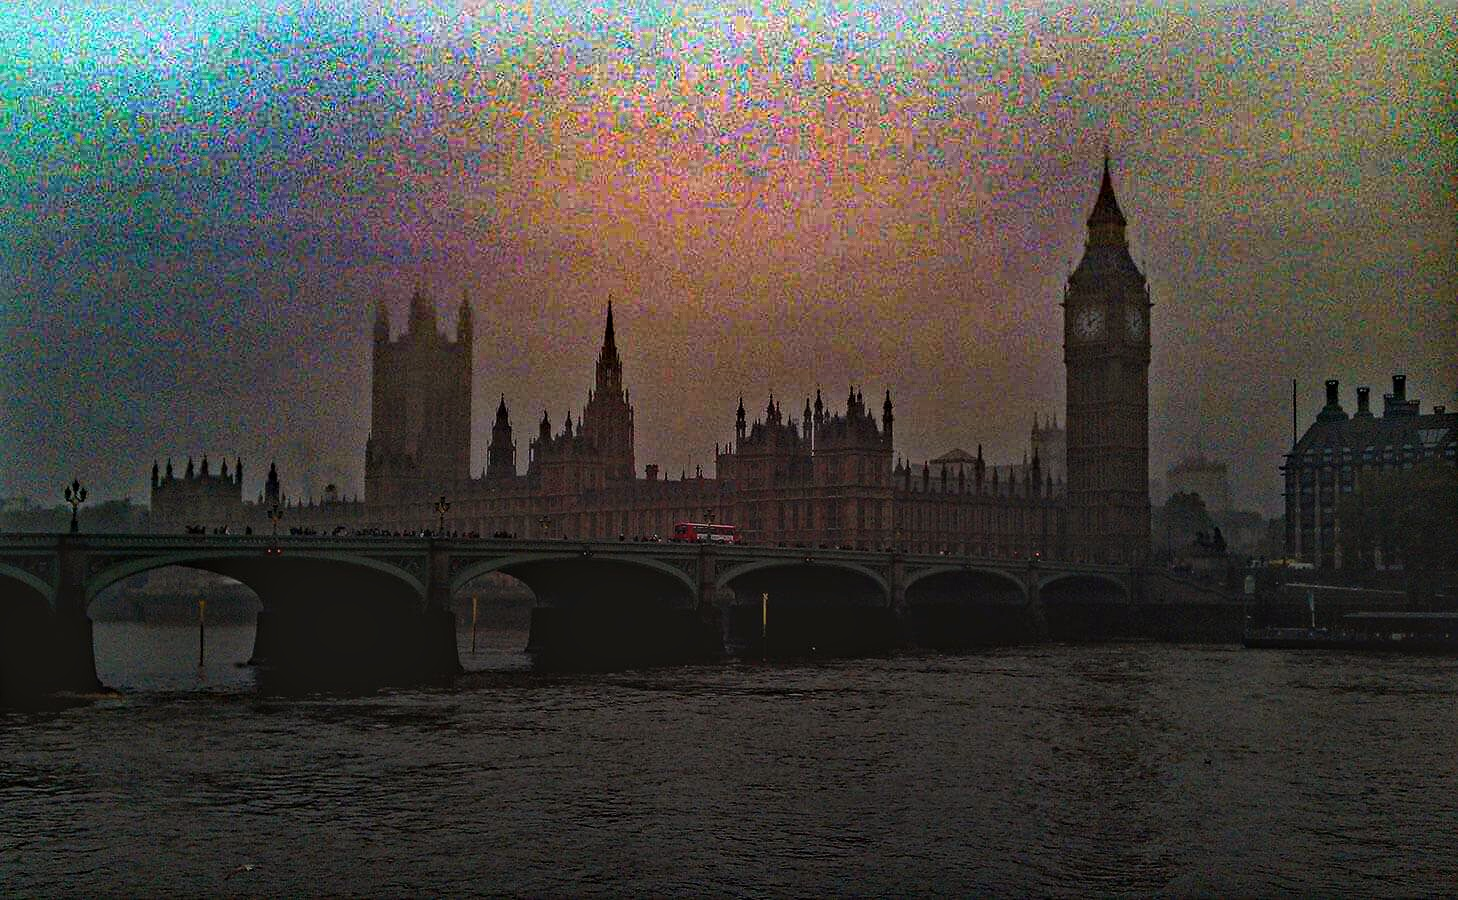
\includegraphics[width=0.3\textwidth]{../output/HSTS_real-world/M_HazyDr_Google_396.jpeg}}
    \\
    \subfloat[CEP]{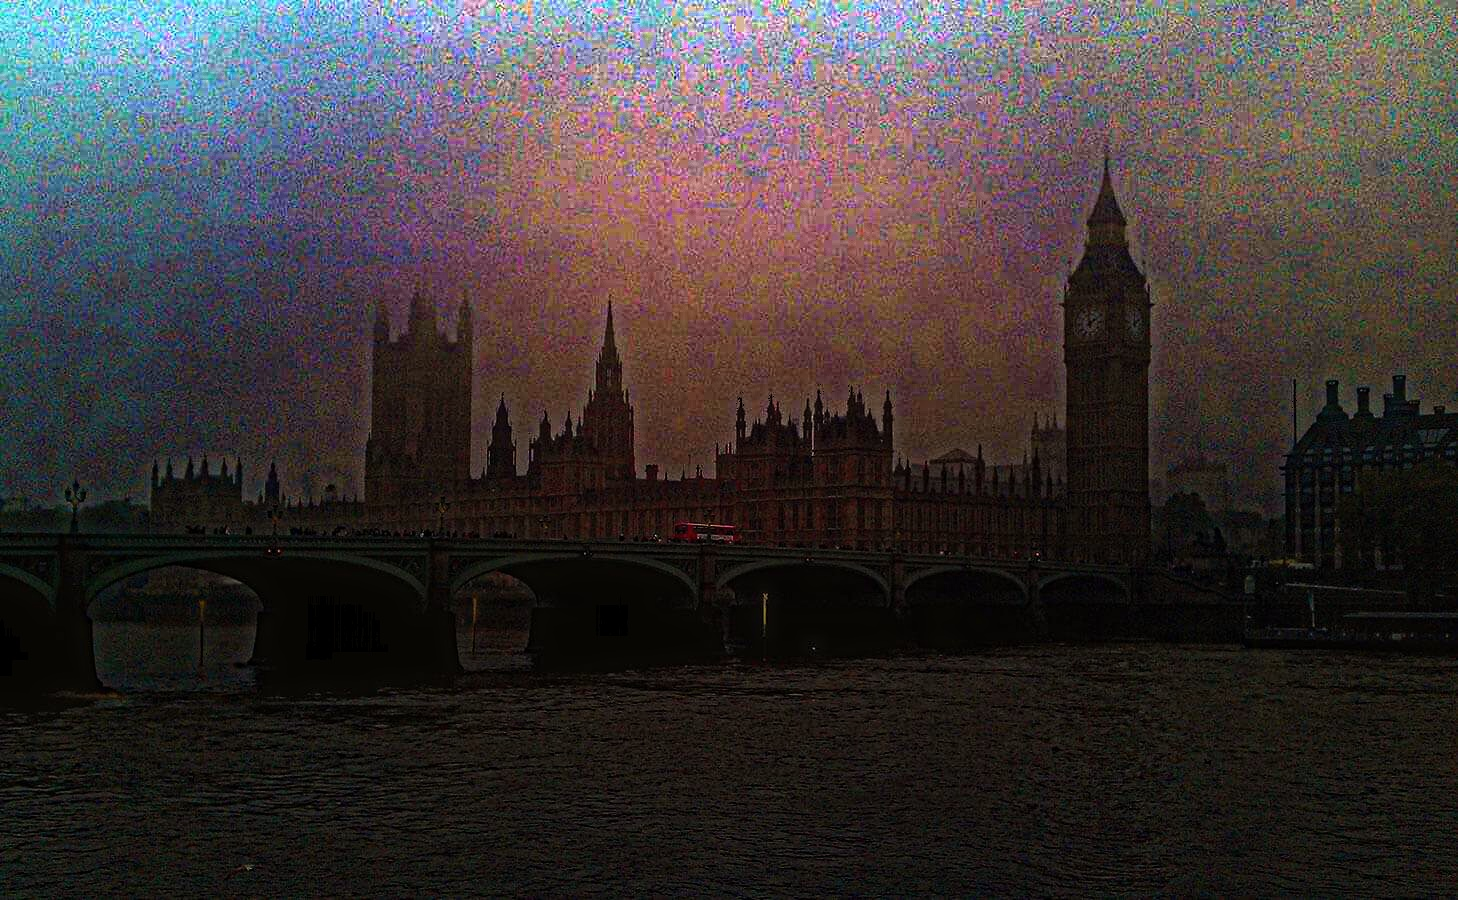
\includegraphics[width=0.3\textwidth]{../output/HSTS_real-world/CEP_HazyDr_Google_396.jpeg}}\quad
    \subfloat[CEP-fast]{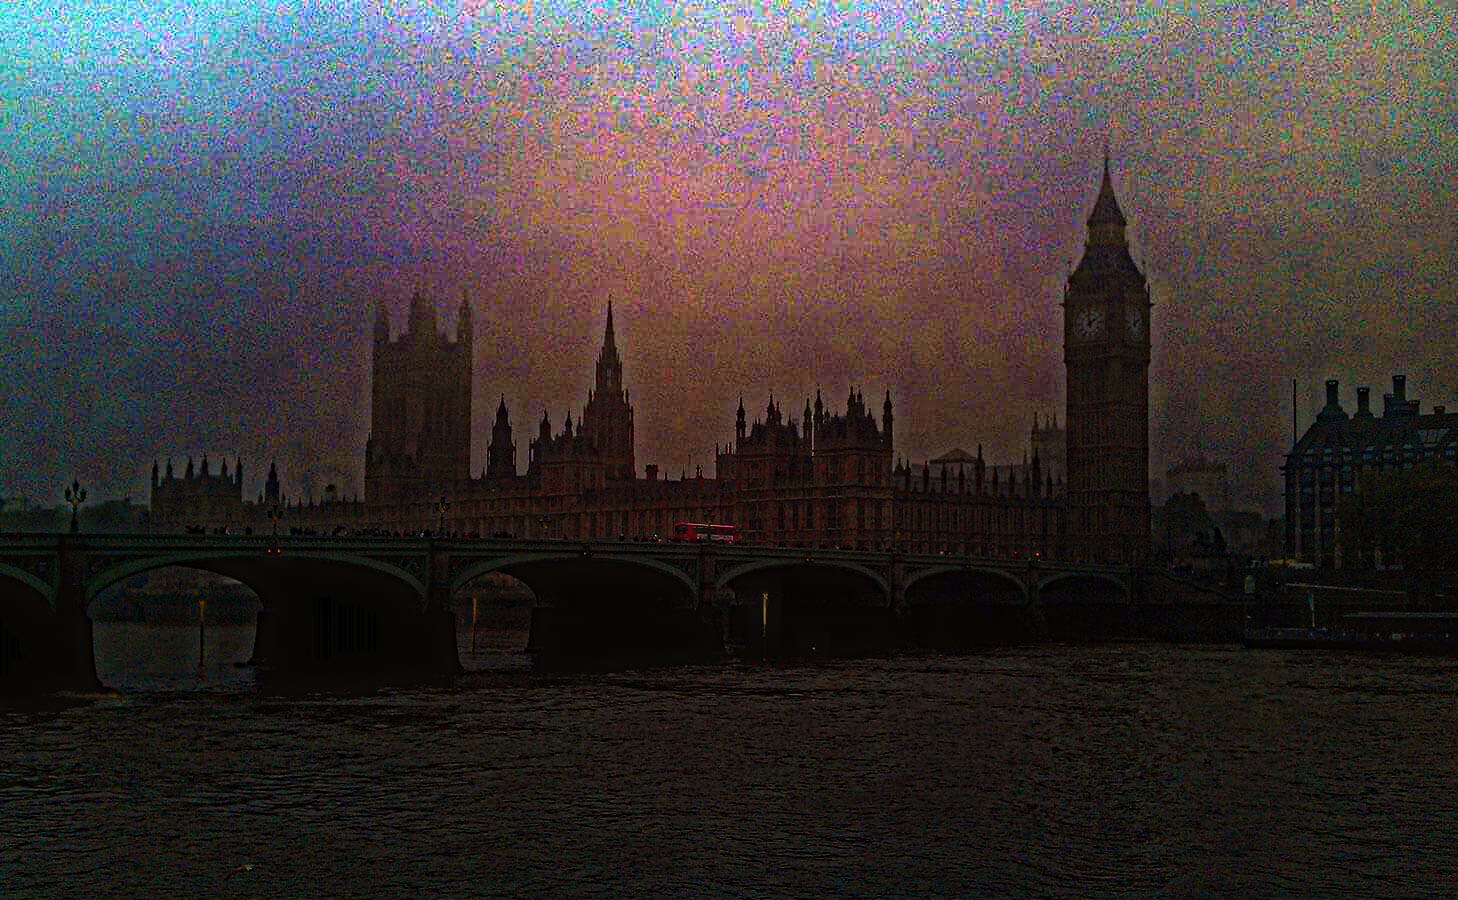
\includegraphics[width=0.3\textwidth]{../output/HSTS_real-world/CEPf_HazyDr_Google_396.jpeg}}
    \quad\subfloat[NLB]{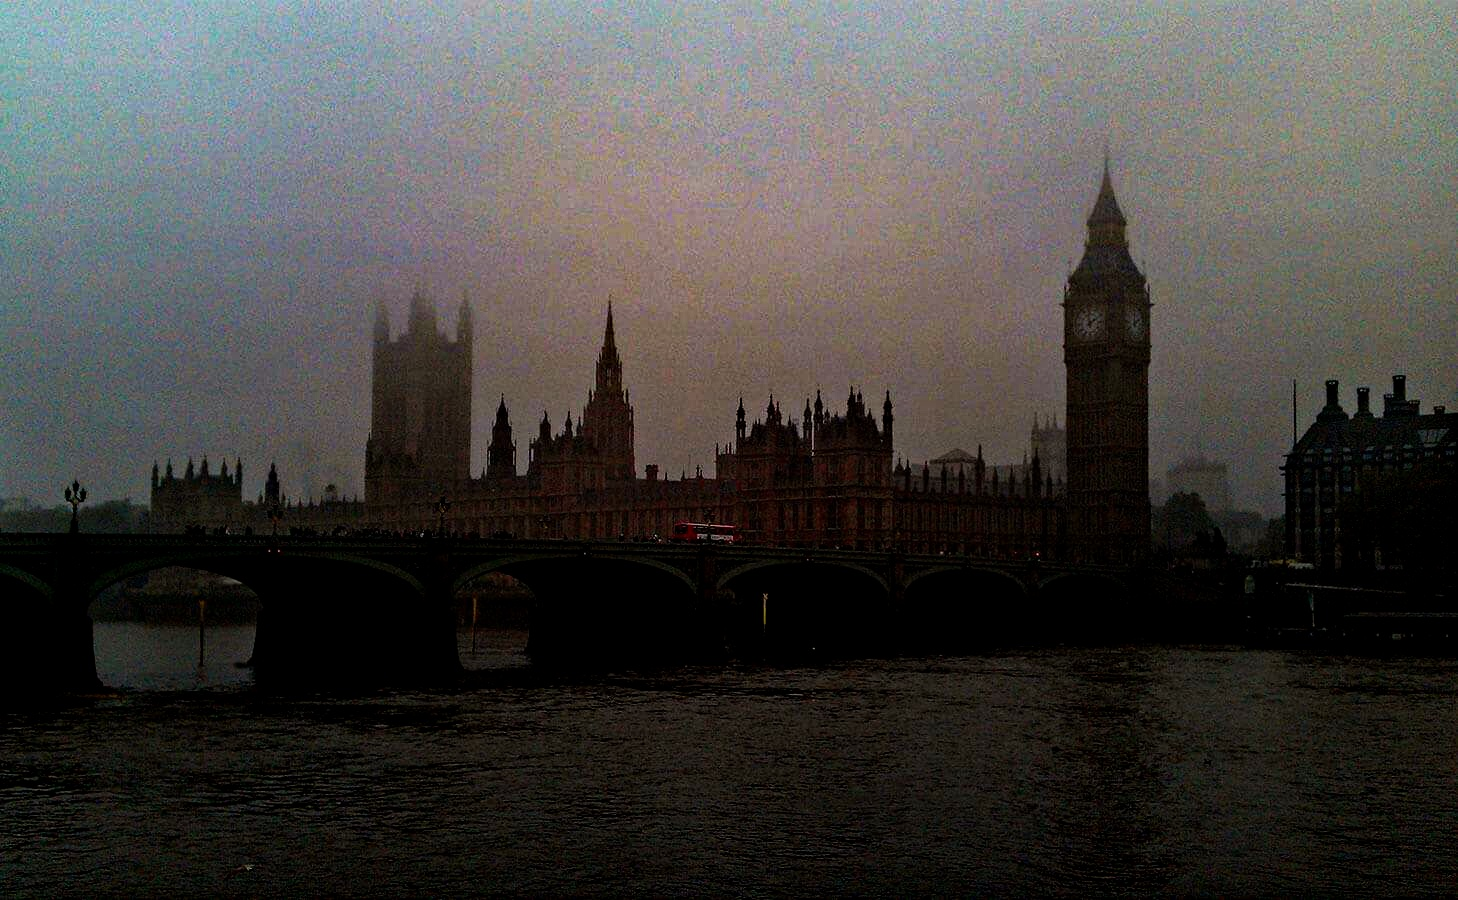
\includegraphics[width=0.3\textwidth]{../output/HSTS_real-world/R_HazyDr_Google_396.jpeg}}
    \\
    \caption{去雾算法结果对比\label{fig-dehazy-cmp}}
\end{figure}

\subsection{客观评价}

\begin{table}
    \caption{SOTS-outdoor数据集下的各算法平均PSNR以及SSIM对比\label{table-cmp}}
    \centering
    \renewcommand{\arraystretch}{2.5} 
    \begin{tabular}{ccc}
        \toprule
        算法 &  PSNR & SSIM \\
        \midrule
        DCP  & $16.9763$ &   $0.8579$  \\
        BCL  & $13.9201$ & $0.7707$\\
        CEP                 & $13.1408$ & $0.6945$\\
        CEP(fast)           & $12.9593$ & $0.6858$\\
        NLB & $14.7957$ & $0.6584$ \\
        \bottomrule
    \end{tabular}
\end{table}

从表\ref{table-cmp}中我们可以获知不同算法在SOTS-outdoor数据集的PSNR与SSIM表现,从表中我们可以获知,复现结果相对合理,与原图由较高的相似性。但是由于没有怎么调整超参数,因此本文复现的效果可能与原文展现的相差甚远,各算法在原文的对比关系可能不太成立,本文复现效果不佳可以归咎于没有像超参,我曾调整过NLB在去雾步骤的$\delta$参数,两个指标都能提升一大截,由于时间不足,没空精调了,为本课程的大作业留下一个遗憾。

